\cleardoublepage
% \newpage
% \thispagestyle{empty}
% \mbox{}

\chapter{Optimización del rendimiento de OmpSs sobre arquitecturas asimétricas}
\label{ch:chapter4}

%\section{Descripción de la estrategia de optimización}
%
%\section{BLIS}
%
%\subsection{Adaptación de BLIS a arquitecturas asimétricas}
%
%\section{Combinación de BLIS asimétrico con OmpSs}
%
\section{Planteamiento y objetivos generales}

(Plantear objetivos e idea general. En el capítulo 5, copiaremos esta estructura, con la
misma sección inicial de motivación/objetivos).

In this section, we initially perform an evaluation 
of the task-parallel Cholesky routine in Listings~\ref{lst:chol}--\ref{lst:chol_tasks},
executed on top of the conventional (i.e., default) scheduler in 
OmpSs linked to a sequential instance of BLIS,  on the target Exynos 5422 SoC.  The outcome from this study 
motivates the development effort and experiments presented in the remainder of the paper.

\subsection{Evaluación de runtimes convencionales en AMPs}

La Figura~\ref{fig:ompss_blis_oversubscription} muestra el rendimiento, en términos de GFLOPS (miles de millones de
operaciones en coma flotante por segundo), mostrado por el runtime convencional de OmpSs para la factorización
de Cholesky, variando el número de \wts entre~1 y~8 sobre la plataforma asimétrica \odroid; en el 
experimento, se delega la asignación de \wts a núcleos al planificador del sistema operativo. En otras palabras,
se está utilizando una versión no consciente de la asimetría del planificador de tareas en OmpSs.
Para este experimento, se ha evaluado un rango lo suficientemente amplio de tamaños de bloque 
({\tt b} en el código de la Figura~\ref{lst:chol}), aunque por simplicidad se reporta únicamente los
resultados obtenidos para el valor de {\tt b} que optimiza el ratio de GFLOPS para cada dimensión
del problema\footnote{En este capítulo, todos los exprimentos se han realizado utilizando doble precisión.}.

\begin{figure}
\centering
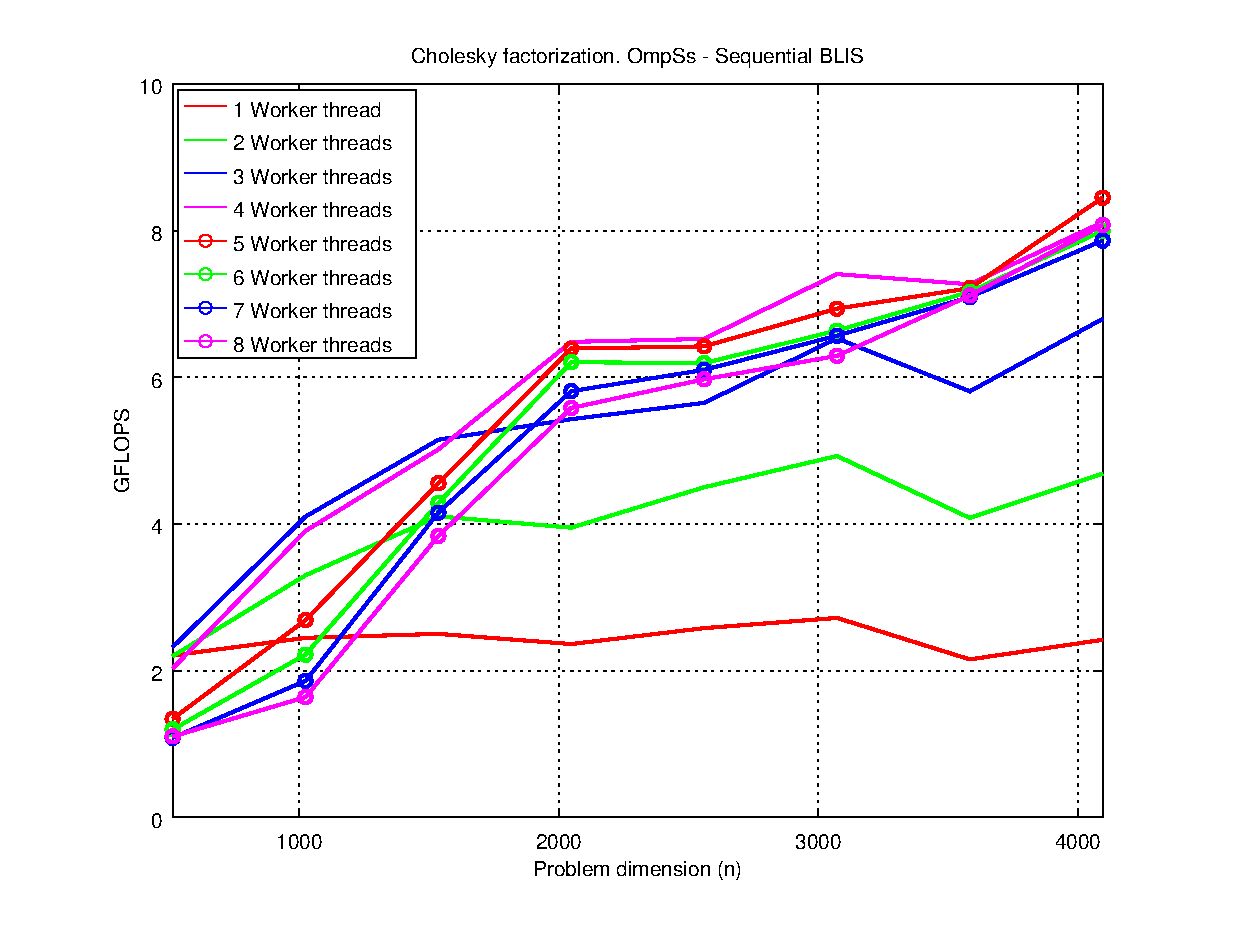
\includegraphics[width=0.70\textwidth]{Plots/Orig_runtime/plot_1to8_th}
\caption{Rendimiento de la factorización de Cholesky utilizando el runtime OmpSs convencional y una implementación secuencial
	de BLIS sobre el SoC Exynos 5422.}
\label{fig:ompss_blis_oversubscription}
\end{figure}

%All the experiments hereafter employed {\sc ieee} double precision. Furthermore,
%we  ensured that the cores operate at the highest possible frequency by setting the appropriate {\em cpufreq} governor.
%The conventional runtime of OmpSs corresponds to release 15.06 of the Nanos++ runtime task scheduler.
%For this experiment, it is lined with the ``sequential'' implementation of BLIS in release 0.1.5.
%(For the experiments with the multi-threaded/asymmetric version of BLIS in the later sections, 
%we will use specialized versions of the codes in~\cite{asymBLIS} for slow+fast VCs.)

Los resultados experimentales revelan un incremento en el rendimiento a medida que el número de \wts aumenta entre~1 y~4,
casos en los que el planificador del sistema operativo asigna su ejecución a los núcleos rápidos (Cortex-A15) disponibles.
Sin embargo, cuando el número de \wts excede la cantidad de núcleos rápidos, el sistema operativo se ve forzado a asignar
\wts a núcleos lentos (Cortex-A7), en cuyo caso el aumento en prestaciones desaparece, e incluso éstas disminuyen drásticamente 
a medida que el número de \wts aumenta. La principal causa de este decremento en las prestaciones es el desequilibrio de carga,
ya que tareas con granularidad univorme, posiblemente pertenecientes al camino crítico, son asignadas a núcleos lentos.

Este experimento revela la principal motivación por la que es necesario un planificador de tareas consciente de la
arquitectura y adaptado a ella~\cite{OmpSsbigLITTLE}. Sin embargo, en el presente capítulo, se desarrollará un enfoque alternativo
a la hora de explotar la asimetría de la arquitectura subyacente: se utilizará un planificador de tareas convencional en combinación
con una biblioteca asimétrica para la ejecución de tareas, como se describe a continuación.

\section{Combinación de runtimes convencionales con bibliotecas asimétricas}

\subsection{Visión general de la propuesta}

La propuesta de operación introducida en el presente capítulo opera bajo el modelo GTS, pero está en cierto modo 
inspirada en el modelo CPUM (véase Sección~\ref{sec:models}). Más concretamente, el objetivo es que el planificador
de tareas considere la arquitectura \odroid (por ejemplo) como una arquitectura verdaderamente simétrica, formada por 
cuatro VCs (núcleos virtuales, o {\em Virtual Cores}), cada uno de ellos compuesto por un núcleo rápido y un núcleo
lento. Para ello, a diferencia del modelo CPUM, {\em ambos} núcleos físicos dentro de cada VC se mantendrán activos y 
colaborarán en la ejecución de una determinada tarea. Así, la propuesta explota dos niveles de concurrencia: el {\em paralelismo
a nivel de tareas} es extraído por el planificador para asignar tareas a cda uno de los cuatro VCs idénticos disponibles en
el sistema, e internamente, cada tarea/kernel divide su carga de forma correcta para exponer {\em paralalismo a nivel de datos}, 
distribuyendo la carga de trabajo entre los dos núcleos físicos asimétricos dentro del VC que está a cargo de la ejecución
de dicha tarea.

Esta solución requiere únicamente un planificador de tareas convencional (es decir, no consciente de la asimetría de la arquitectura, o lo
que es lo mismo, orientado a arquitecturas SMT), como por ejemplo el planificador de tareas convencional proporcionado por OmpSs, donde, 
en lugar de crear un \wt\ por núcleo físico del sistema, se sigue una filosofía similar a la propuesta por el modelo CPUM, creando 
{\em un único worker thread por VC}. Internamente, cuando una tareai es elegida para ser ejecutada por un \wt disponible, dicha tarea
se ejecutará, de forma ya no secuencial, sino paralela sobre cada uno de los núcleos que componen el VC, explotando, en este caso,
la asimetría interna de dicha abstracción. Por ejemplo, en el caso de \odroid, equipada con cuatro núcleos rápidos y cuatro lentos, 
la propuesta desarrollada desplegará únicamente cuatro \wt; para cualquier tarea básica o kernel de álgebra lineal a ejecutar, dicha
rutina explotará la asimetría internamente, siempre bajo la condición de que existe una implementación de la misma optimizada para
este tipo de paralelismo asimétrico.

Siguiendo esta idea, la arquitectura expuesta al planificador de tareas es completamente {\em simétrica}, y los kernels en BLIS
(o en cualquier otra biblioteca utilizada para la ejecución de las tareas) configuran una ``caja negra'' que abstrae del carácter
asimétrico al planificador.

En resumen, si en una configuración convencional el núcleo es el recurso mínimo de computación para el planificador de tareas,
y éstas son totalmente secuenciales, en la solución propuesta el VC es el recurso básico de computación de cara al planificador,
mientras que la implementación de las tareas pasa a ser no sólo paralela, sino adaptada para la correcta explotación del paralelismo
existente dentro de cada VC.

\subsection{Comparación y ventajas frente a otras alternativas}


%Provided an underlying asymmetry-aware library is available to the developer, it is possible to combine this 
%with an existing conventional runtime task scheduler in order to exploit the underlying architecture. 
%In the enhanced version of OmpSs in~\cite{OmpSsbigLITTLE}, tasks were actually invocations to a {\em sequential} 
%library implementation, and asymmetry was exploited via sophisticated scheduling policies specially designed for asymmetric architectures. 
%Following our new approach, asymmetry is exploited at the library level, not at the runtime level. 
%To accommodate this, tasks are cast in terms of 
%invocations to a multi-threaded asymmetry-aware library (in our case, BLIS). 

La solución desarrollada reúne un conjunto de ventajas de cara al desarrollador:

\begin{itemize}
\item El planificador de tareas no es consciente de la asimetría, por lo que cualquier versión convencional 
      del mismo podrá trabajar sobre este tipo de sistemas sin modificaciones específicas. 
\item Cualquier política de planificación (por ejemplo, {\em work stealing}, planificación consciente de la localidad de datos,
      implementación de caches por software, \ldots) ya desarrollada para arquitecturas simétricas, o cualquier futura mejora,
      tendrá también un impacto directo en el rendimiento sobre el sistema asimétrico.
\item Cualquier mejora en la implementación de las bibliotecas asimétricas subyacentes (por ejemplo, BLIS) tendrá un impacto directo
      sobre el AMP. Esta observación se aplica a arquitecturas con distinto número de núcleos lentos/rápidos dentro del VC, ratios
      en las frecuencias de funcionamiento, o incluso ante la introducción de más niveles de asimetría (esto es, núcleos con rendimiento
      intermedio).
\end{itemize}

Obviamente, existe una dificultad adicional intrínseca a la solución propuesta, y que se convierte en un requisito fundamental de cara
a su viabilidad: debe existir, necesariamente, una versión conscente de la asimería para cada tarea a ejecutar (por ejemplo, una implementación
completa de las rutinas BLAS). En el ámbito del álgebra lineal densa, este requisito se cumple a través de la versión asimétrica de BLIS, aunque
en otros ámbitos, el desarrollo específico de este tipo de implementaciones es todavía escaso.

\subsection{Requisitos a nivel de tarea en el ámbito del álgebra lineal}

\comentario{Hay que reescribir esta sección}.

Por último, cabe destacar que son necesarios ciertos requisitos adicionales en la implementación multihebra de BLIS
que opera sobre el modelo propuesto. Considérese el kernel \gemm y la descripción de alto nivel proporcionada en la Figura~\ref{lst:gemm}. 
Como se ha descrito anteriormente, resulta necesario distribuir el espacio de iteraciones de alguno de los bucles entre los dos tipos de núcleos
que conforman un VC; siguiendo las directivas de paralelización descritas en~\cite{BLIS3}, se distinguen a continuación dos escenarios de reparto posibles:

\begin{itemize}
	\item En arquitecturas donde cada VC está compuesto por igual número de núcleos de cada tipo (por ejemplo, \odroid) \ldots

	\item En arquitecturas donde cada VC está compuesto por distinto número de núcleos de cada tipo (por ejemplo, \juno) \ldots

\end{itemize}

For our objective, we still have to distribute the iteration space between the Cortex-A15 and the Cortex-A7 but, since there is only one resource of each type per VC,
there is no need to partition the loops internal to the macro-kernel. 
Furthermore, we note that the optimal strides for Loop~1 are in practice quite
large ({\tt nc} is in the order of a few thousands for ARM big.LITTLE cores), while the optimal values for Loop~3 are much more reduced
({\tt mc} is 32 for the Cortex-A7 and 156 for the Cortex-A15). Therefore, we target Loop~3 in our data-parallel implementation of BLIS for
VCs, which we can expect to easily yield a proper workload balancing.

%That is, both the number of cores to use, and the distribution of those cores between the fast and slow processing units are transparent and 
%fully configurable by the user. 

\section{Resultados experimentales}

\subsection{Estudio experimental del tamaño de bloque óptimo}

En tiempo de ejecución, OmpSs descompone la rutina para la implementación de la factorización de Cholesky en una colección de tareas
que operan en submatrices (bloques) con una granularidad que viene definida por el tamaño de bloque {\tt b}, véase el código en la 
Figura~\ref{lst:chol}. Estas tareas típicamente se reducen a invocaciones a kernels elementales a nivel de BLAS (en nuestro caso,
BLIS) o LAPACK, véase el código proporcionado en la Figura~\ref{lst:chol_tasks}.  

\newcommand{\bopt}{b^{\mbox{\rm \scriptsize opt}}\xspace}

El primer paso en nuestra evaluación radica en proporcionar una estimación realista de la ganancia de rendimiento
potencial proporcionada por la solución propuesta (en caso de haberla). Un factor crítico desde este punto de vista es
el rango de tamaños de bloque que resultan óptimos para el runtime convencional de OmpSs ante una determinada operación
(en adelante $\bopt$). En particular, la eficiencia de la solución propuesta vendrá determinada por el rendimiento obtenido
por las implementaciones BLIS de cada una de las tareas que componen la operación, comparada con su implementación secuencial
equivalente para dimensiones del problema {\tt n} en el orden de dimensión $bopt$.

La Tabla~\ref{tab:optimal_bs_sym} muestra los tamaños de bloque óptimos $\bopt$ para la factorización de Cholesky y tamaños
de problema crecientes, utilizando el planificador OmpSs convencional enlazado con una versión secuencial de BLIS y un número
creciente de \wts entre~1 y~4. Obsérvese como, excepto para los menores tamaños de problema, los tamaños de bloque óptimos están
en el rango entre 192 y 448. Estos tamaños de bloque resultan óptimos al ofrecer un equilibrio entre el paralelismo a nivel de tareas
potencial y la eficiencia interna de las ejecuciones secuenciales de cada tarea individual.

\newcommand{\ra}[1]{\renewcommand{\arraystretch}{#1}}
\newcommand{\ca}[1]{\renewcommand{\tabcolsep}{#1}}

\ra{1.2}
\ca{2pt}

\begin{table}
	\centering
	\caption{Tamaños de bloque óptimos para la factorización de Cholesky utilizando el planificador convencional
	         de OmpSs y una implementación secuencial de BLIS sobre \odroid.}
	\label{tab:optimal_bs_sym}
{\scriptsize
\begin{tabular}{crrrrrrrrrrrrrrrr} 
\toprule
  & \phantom{a} & \multicolumn{14}{c}{Tamaño del problema ({\tt n})} \\ 
\cmidrule{3-17} 
  & \phantom{a} &     512 & 1,024 & 1,536 & 2,048 & 2,560 & 3,072 & 3,584 & 4,096 & 4,608 & 5,120 & 5,632 & 6,144 & 6,656 & 7,168 & 7,680 \\ \hline

{\sc 1 wt} & \phantom{a} &     192 & 384  & 320  & 448  & 448  & 448  & 384  & 320 & 320 & 448 & 448 & 448 & 448 & 384 & 448 \\ \hline
{\sc 2 wt} & \phantom{a} &     192 & 192  & 320  & 192  & 448  & 448  & 384  & 320 & 320 & 448 & 448 & 448 & 448 & 384 & 448 \\ \hline
{\sc 3 wt} & \phantom{a} &     128 & 192  & 320  & 192  & 384  & 448  & 320  & 320 & 320 & 448 & 448 & 448 & 448 & 384 & 448 \\ \hline
{\sc 4 wt} & \phantom{a} &     128 & 128  & 192  & 192  & 192  & 320  & 320  & 320 & 320 & 448 & 320 & 448 & 448 & 384 & 448 \\ \bottomrule
\end{tabular}
}
\end{table}

La principal conclusión extraída tras el análisis de los resultados es la siguiente: para elevar el rendimiento de un planificador
de tareas combinado con una versión asimétrica de BLIS, cada uno de los kernels que componen la operación implementados en dicha
versión asimétrica debe exhibir mayor rendimiento que las respectivas implementaciones secuenciales, para dimensiones de matrices 
que estén en el orden de los tamaños de bloque mostrados en la Tabla~\ref{tab:optimal_bs_sym}.  

La Figura~\ref{fig:cross_blis} muestra el rendimiento alcanzado para las tres rutinas básicas BLAS que componen la factorización
de Cholesky (\gemm, \syrk y \trsm) para el rango de dimensiones de interés sobre la plataforma \odroid.  
El experimento compara la versión secuencial de BLIS sobre un único núcleo Cortex-A15 con la versión asimétrica de BLIS
que combina un Cortex-A15 y un Cortex-A7. Es decir, compara la ejecución de las tareas que componen la factorización sobre un
único núcleo físico (rápido) y sobre un VC (combinando un núcleo rápido y otro lento).

En general, las tres rutinas BLAS muestran una tendencia similar: los kernels de la versión secuencial de BLIS
consiguen mejor rendimiento que sus respectivas implementaciones asimétricas para tamaños de problema pequeños (hasta
aproximadamente {\tt m}, {\tt n}, {\tt k } = 128); sin embargo, 
a partir de dicha dimensión, el uso de un núcleo lento comienza a hacer que el rendimiento mejore. 
El aspecto más importante radica en el hecho de que el punto de corte entre ambas curvas está en el rango (e incluso 
es típicamente menor) de $\bopt$, véase Tabla~\ref{tab:optimal_bs_sym}. 
Esto implica que la versión asimétrica de BLIS puede, potencialmente, mejorar el rendimiento general de la factorización, 
incluso usando un planificador de tareas convencional.
Además, la mejora en rendimento aumenta con el tamaño de problema, estabilizándose para dimensiones alrededor de 
{\tt m}, {\tt n}, {\tt k } $\approx~400$. Dado que este valor está en el randgo del tamaño de bloque óptimo para
la factorización de Cholesky, sobre esta arquitectura es esperable una mejora en el orden de 0.3--0.5 GFLOPS por núcleo lento
añadido.
%mimicking the behavior of the underlying BLIS.

\begin{figure}[t]
\centering
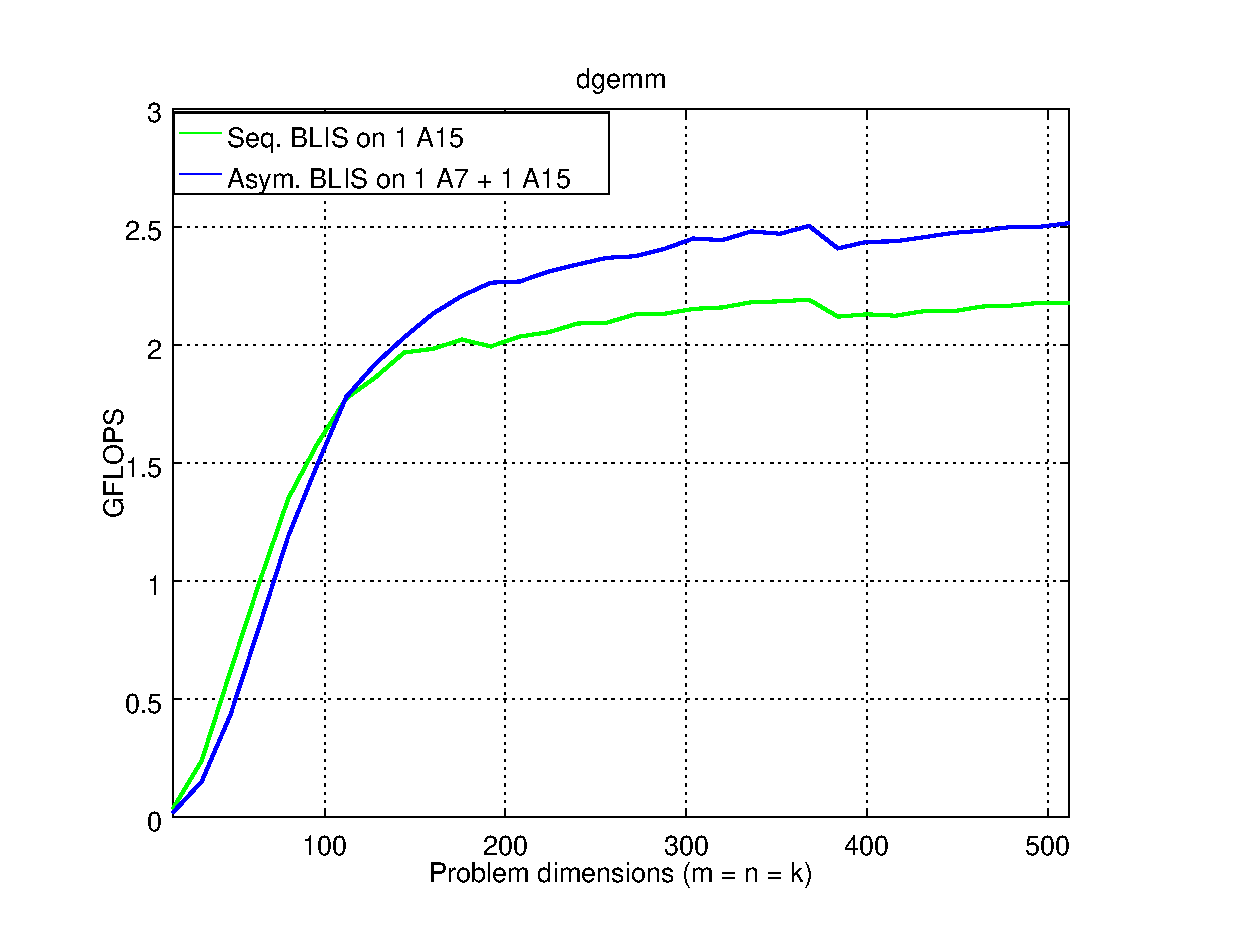
\includegraphics[width=0.49\textwidth]{Plots/BLIS_small/blis_dgemm_sym_asym}
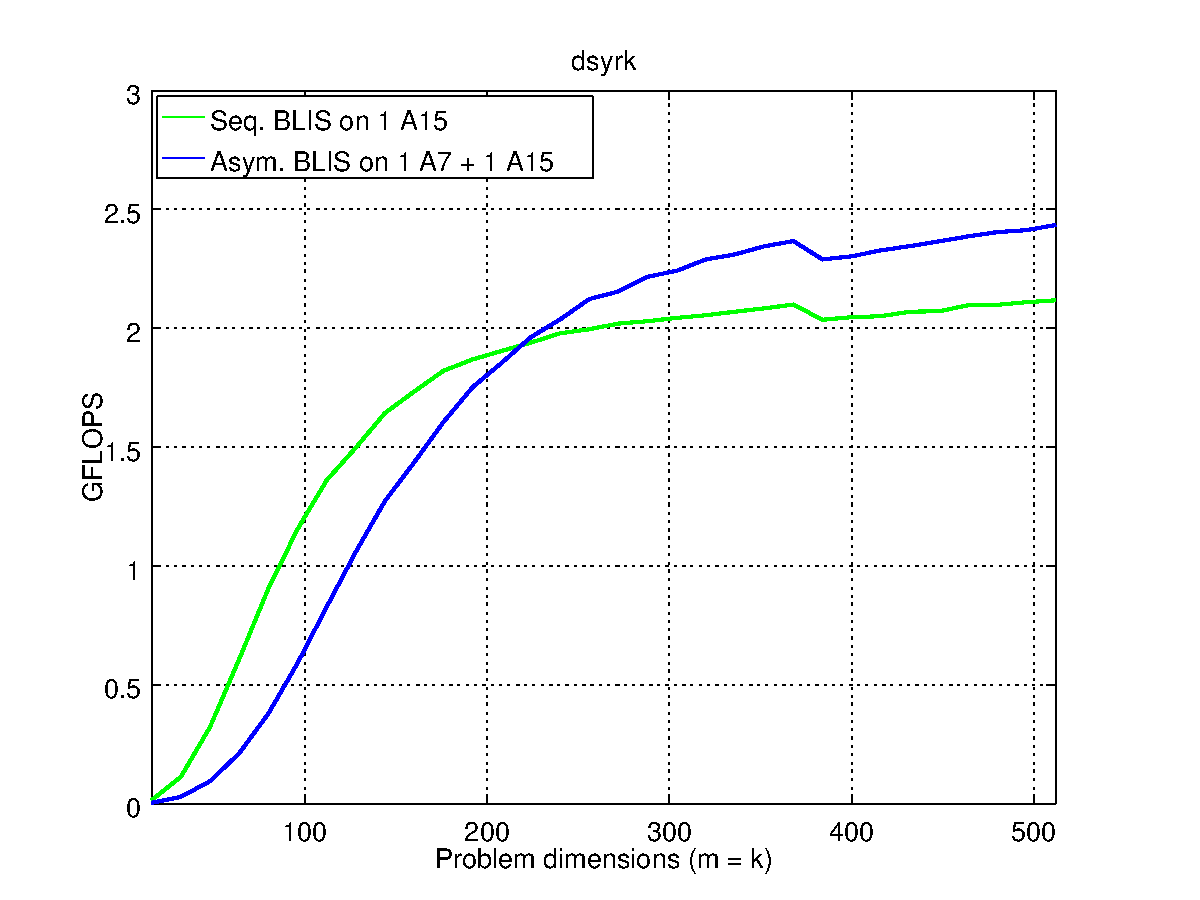
\includegraphics[width=0.49\textwidth]{Plots/BLIS_small/blis_dsyrk_sym_asym}
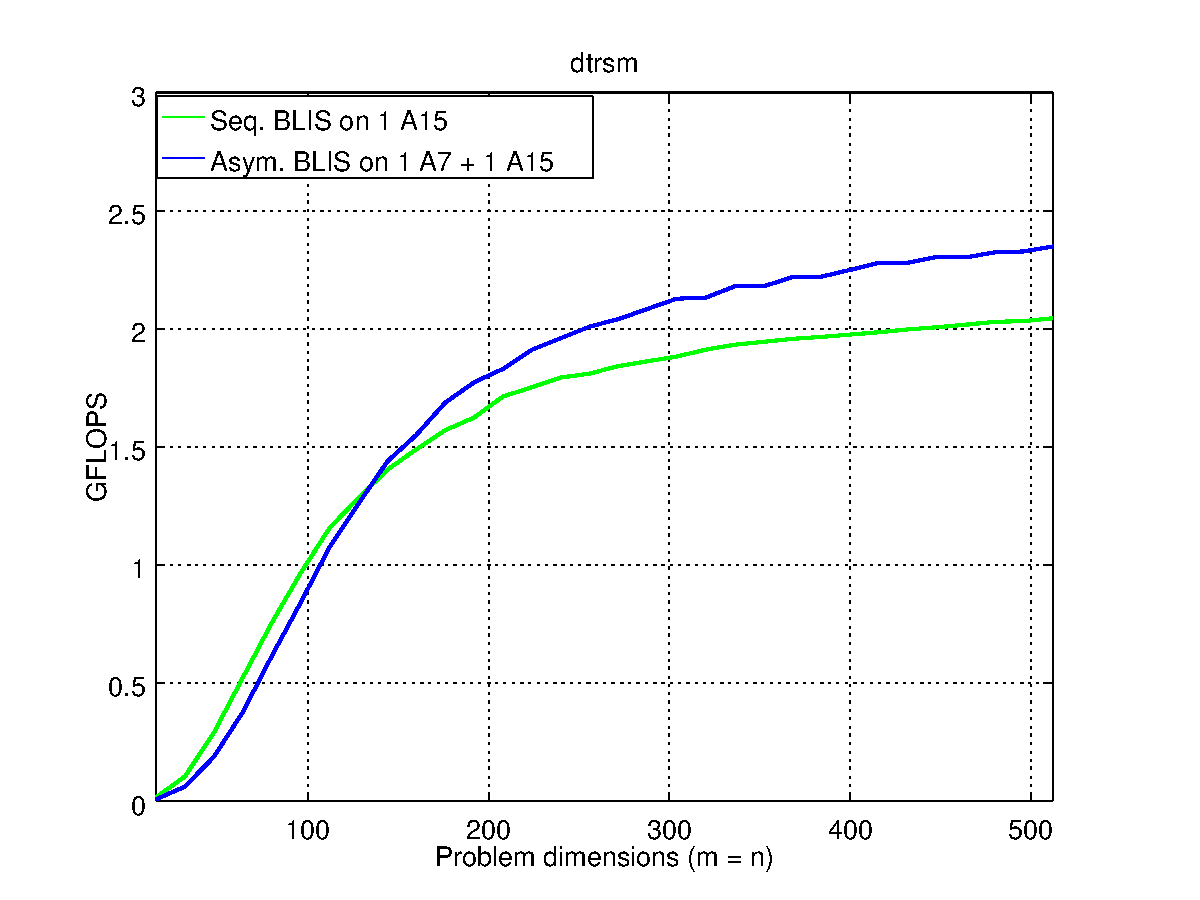
\includegraphics[width=0.49\textwidth]{Plots/BLIS_small/blis_dtrsm_sym_asym}
\caption{Rendimiento de los kernels BLAS-3 en las implementaciones secuencial y asimétrica de BLIS, utilizando, respectivamente
         un núcleo Cortex-A15 y un núcleo Cortex-A15 más un núcleo Cortex-A7 sobre \odroid.}
\label{fig:cross_blis}
\end{figure}


\subsection{Integración de BLIS asimétrico con un planificador de tareas convencional}

Con el fin de analizar los beneficios reales de la solución propuesta en términos de rendimiento, comparamos a continuación
el rendimiento del planificador OmpSs enlazado con {\em (a)} una versión secuencial de BLIS, y {\em (b)} con la versión asimétrica de BLIS. 
En todos los experimentos, los kernels BLIS en la primera configuración utlilizarán exclusivamente un núcleo Cortex-A15, mientras
que en el segundo caso se utlizará un núcleo Cortex-A15 más un núcleo Cortex-A7 para la ejecución de las tareas.
%
La Figura~\ref{fig:ompss_blis} muestra los resultados obtenidos para ambas configuraciones, utilizando un número creciente
de \wts, entre~1 y~4. Por simplicidad, únicamente se reportan los resultados obtenidos considerando el tamaño de bloque óptimo
para cada tamaño de problema. En todos los casos, la solución basada en la utilización de una bilioteca asimétrica mejora
el rendimiento de la implementación secuencial para matrices relativamente grandes (típicamente con dimensiones {\tt n}~$>$~2,048)
mientras que, para tamaños de problema menores, el ratio de GFLOPS obtenido en ambos casos es similar. 
La razón de este comportamiento viene marcada por el tamaño de bloque óptimo reportado en la Tabla~\ref{tab:optimal_bs_sym}
y el rendimento de BLIS mostrado en la Figura~\ref{fig:cross_blis}: para dicho rango de dimensiones de problema,
el tamaño óptimo de bloque es significativamente menor, y ambas implementaciones BLIS obtienen resultados de rendimiento similares.

\begin{figure}%[t]
\centering
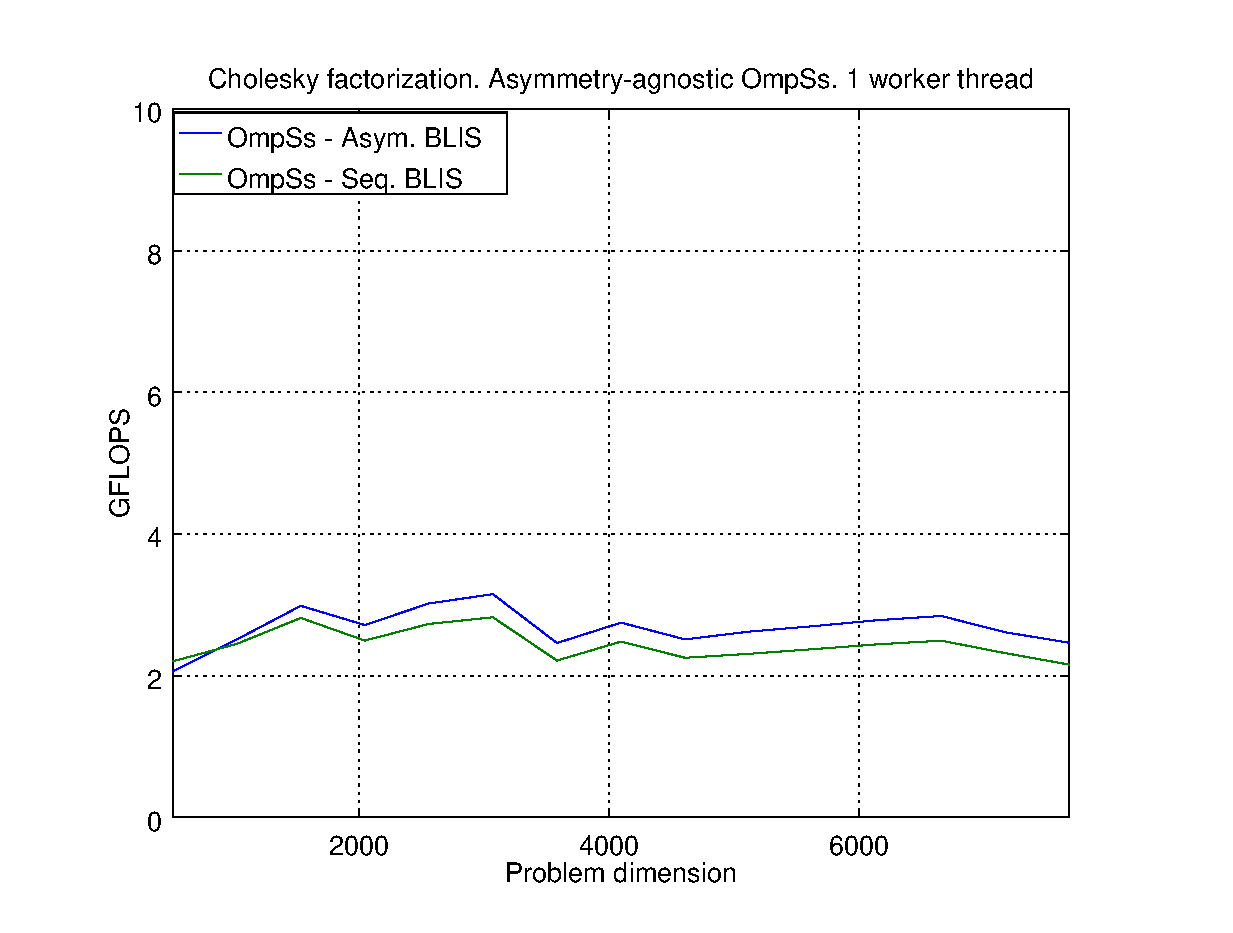
\includegraphics[width=0.49\textwidth]{Plots/Orig_runtime/plot_1_th}
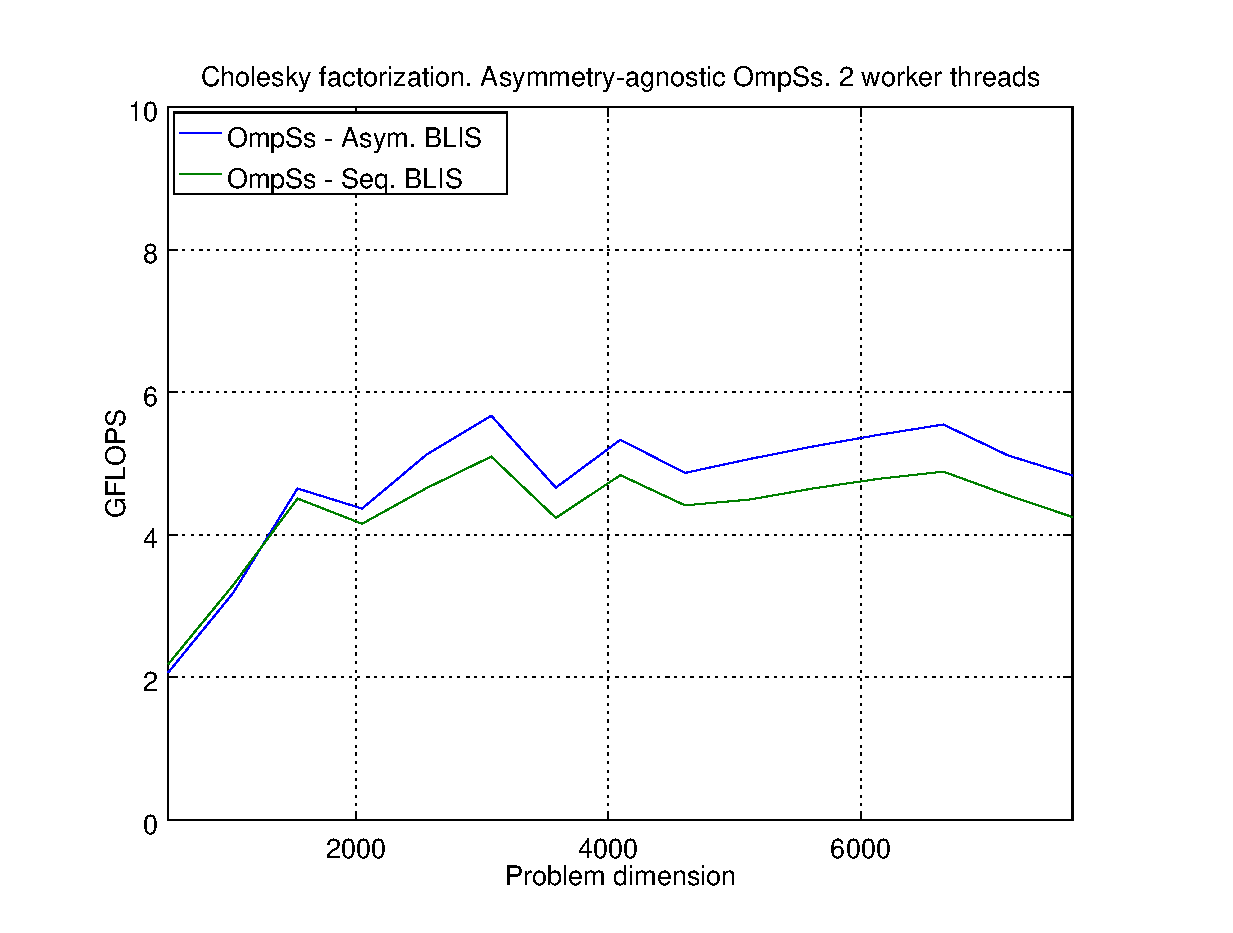
\includegraphics[width=0.49\textwidth]{Plots/Orig_runtime/plot_2_th}
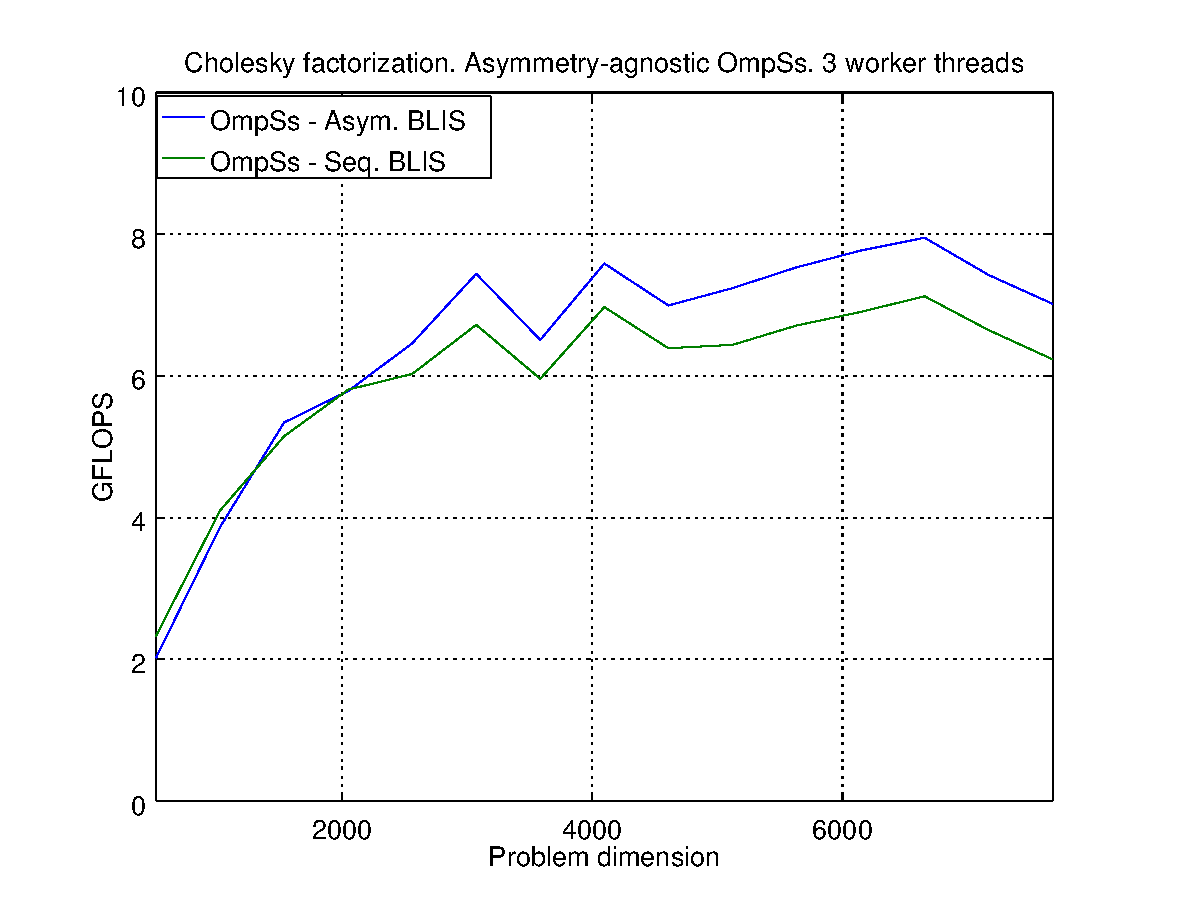
\includegraphics[width=0.49\textwidth]{Plots/Orig_runtime/plot_3_th}
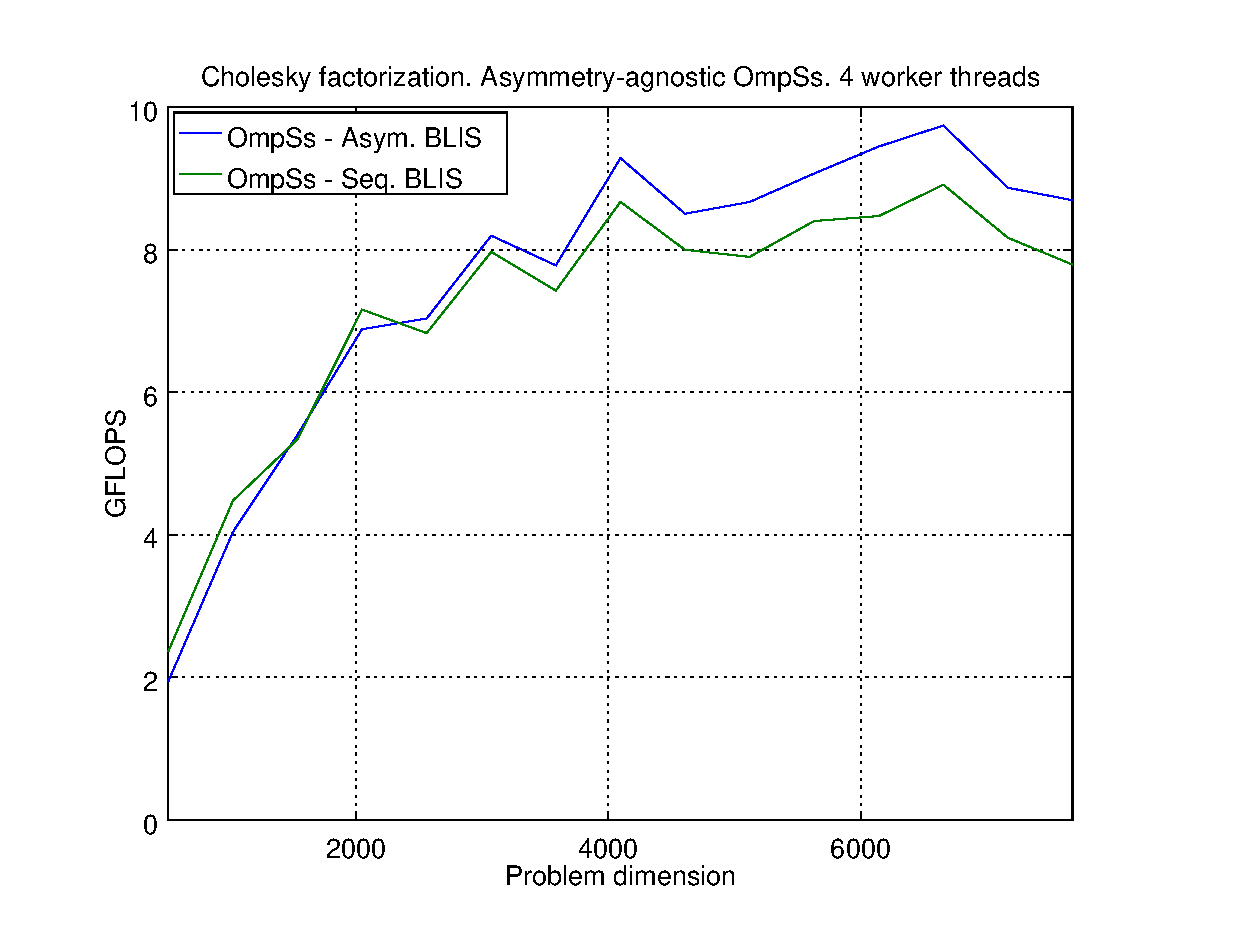
\includegraphics[width=0.49\textwidth]{Plots/Orig_runtime/plot_4_th}
\caption{Rendimiento de la factorización de Cholesky utilizando el planificador convencional de OmpSs, enlazado
         con la versión secuencial y asimétrica de BLIS.}
\label{fig:ompss_blis}
\end{figure}


%Table~\ref{tab:optimal_bs_sym}\ldots
%
%\begin{table}
	%\centering
	%\caption{Optimal block sizes for the Cholesky factorization using asymmetric BLIS.}
	%\label{tab:optimal_bs_asym}
	%\begin{tabular}{|c||c|c|c|c|c|c|c|c|c|c|c|c|c|c|c|}
		%\hline
		 %Th. &    512 & 1024 & 1536 & 2048 & 2560 & 3072 & 3584 & 4096 & 4608 & 5120 & 5632 & 6144 & 6656 & 7168 & 7680 \\ \hline \hline
		 %1   &    192 & 384 & 320 & 448 & 448 & 448 & 384 & 320 & 448 & 448 & 448 & 448 & 448 & 384 & 448 \\ \hline
		 %2   &    192 & 192 & 320 & 320 & 448 & 448 & 384 & 320 & 320 & 448 & 448 & 448 & 448 & 384 & 448 \\ \hline
		 %3   &    192 & 192 & 320 & 192 & 384 & 448 & 384 & 320 & 320 & 448 & 448 & 448 & 448 & 384 & 448 \\ \hline
		 %4   &    192 & 192 & 320 & 192 & 384 & 320 & 320 & 320 & 320 & 448 & 448 & 448 & 448 & 384 & 448 \\ \hline
	%\end{tabular}
%
%\end{table}

The quantitative difference in performance between both approaches is
reported in Tables~\ref{tab:improvement_absolute} and~\ref{tab:improvement_percore}. 
%In both tables, we
%report the difference in performance introduced by the use of an asymmetric BLIS implementation compared with the same setup using sequential BLIS. Table~\ref{tab:improvement_absolute} 
The first table illustrates the raw (i.e., absolute) gap, while the second
one shows the difference per Cortex-A7 core introduced in the experiment. 
Let us consider, for example, the problem size {\tt n}~=~6,144. 
In that case, the performance roughly improves by 0.975 GFLOPS when the 4~slow cores are added to help the base 4~Cortex-A15 cores. 
This translates into a performance raise of 0.243 GFLOPS per slow core, which is slightly under the 
improvement that could be expected from results experiments in the previous section. 
Note, however, that the performance per Cortex-A7 core is reduced from 0.340~GFLOPS, when adding just one
core, to 0.243~GFLOPS, when simultaneously using all four slow cores.

\newcommand{\fg}[1]{\textcolor{ForestGreen}{#1}} % Verde
\newcommand{\br}[1]{\textcolor{BrickRed}{#1}} % Rojo

\begin{table}
	\centering
\caption{Absolute performance improvement (in GFLOPS) for the Cholesky factorization using
         the conventional OmpSs runtime linked with 
         the multi-threaded/asymmetric BLIS with respect to the same runtime linked with the sequential BLIS in
         the Exynos 5422 SoC.}
	 \label{tab:improvement_absolute}

%\begin{tabular}{|c||c|c|c|c|c|c|c|c|c|c|c|c|c|} 
   	%\hline
	%Th. &        512    & 1024       & 2048     & 2560     & 3072      & 4096     & 4608     & 5120    & 5632    & 6144     & 6656     & 7168     & 7680 \\ \hline \hline
	%1   &     -0.143    & 0.061      & 0.218    & 0.289    & 0.326     & 0.267    & 0.259    & 0.313   & 0.324   & 0.340    & 0.348    & 0.294    & 0.300    \\ \hline
	%2   &     -0.116    & -0.109     & 0.213    & 0.469    & 0.573     & 0.495    & 0.454    & 0.568   & 0.588   & 0.617    & 0.660    & 0.558    & 0.582    \\ \hline
	%3   &     -0.308    & -0.233     & -0.020   & 0.432    & 0.720     & 0.614    & 0.603    & 0.800   & 0.820   & 0.866    & 0.825    & 0.777    & 0.78    \\ \hline
	%4   &     -0.421    & -0.440     & -0.274   & 0.204    & 0.227     & 0.614    & 0.506    & 0.769   & 0.666   & 0.975    & 0.829    & 0.701    & 0.902    \\ \hline
%\end{tabular}
%%\end{table}

\ra{1.2}
\ca{2pt}

{\scriptsize
\begin{tabular}{crrrrrrrrrrrrr} 
   	\toprule
                 & \phantom{a} & \multicolumn{12}{c}{Problem dimension ({\tt n})} \\ 
\cmidrule{3-14} 
     & \phantom{a} &       512      & 1,024        & 2,048          & 2,560        & 3,072        & 4,096        & 4,608        & 5,120        & 5,632        & 6,144        & 6,656         & 7,680 \\ \hline 
{\sc 1 wt} & \phantom{a} &    \br{-0.143} & \fg{0.061}  & \fg{0.218}    & \fg{0.289}  & \fg{0.326}  & \fg{0.267}  & \fg{0.259}  & \fg{0.313}  & \fg{0.324}  & \fg{0.340}  & \fg{0.348}   & \fg{0.300} \\ \cline{3-14}
{\sc 2 wt} & \phantom{a} &    \br{-0.116} & \br{-0.109} & \fg{0.213}    & \fg{0.469}  & \fg{0.573}  & \fg{0.495}  & \fg{0.454}  & \fg{0.568}  & \fg{0.588}  & \fg{0.617}  & \fg{0.660}   & \fg{0.582} \\ \cline{3-14}
{\sc 3 wt} & \phantom{a} &    \br{-0.308} & \br{-0.233} & \br{-0.020}   & \fg{0.432}  & \fg{0.720}  & \fg{0.614}  & \fg{0.603}  & \fg{0.800}  & \fg{0.820}  & \fg{0.866}  & \fg{0.825}   & \fg{0.780} \\ \cline{3-14}
{\sc 4 wt} & \phantom{a} &    \br{-0.421} & \br{-0.440} & \br{-0.274}   & \fg{0.204}  & \fg{0.227}  & \fg{0.614}  & \fg{0.506}  & \fg{0.769}  & \fg{0.666}  & \fg{0.975}  & \fg{0.829}   & \fg{0.902} \\ \bottomrule
\end{tabular}
}
\end{table}


%\begin{table}
	%\centering
	%\caption{Performance improvement per introduced core (in GFLOPS) when using asymmetric BLIS combined with OmpSs for the Cholesky factorization.}
	%\label{tab:improvement_percore}
%
%\begin{tabular}{|c||c|c|c|c|c|c|c|c|c|c|c|c|c|} 
   	%\hline
	 %Th. &       512    & 1024     & 2048     & 2560     & 3072      & 4096     & 4608     & 5120    & 5632     & 6144     & 6656    & 7168     & 7680 \\ \hline \hline
	 %1   &    -0.143    & 0.061    & 0.218    & 0.289    & 0.326     & 0.267    & 0.259    & 0.313   & 0.324    & 0.340    & 0.348   & 0.294    & 0.300    \\ \hline
	 %2   &    -0.058    & -0.054   & 0.106    & 0.234    & 0.286     & 0.247    & 0.227    & 0.284   & 0.294    & 0.308    & 0.330   & 0.279    & 0.291    \\ \hline
	 %3   &    -0.102    & -0.077   & -0.006   & 0.144    & 0.240     & 0.204    & 0.201    & 0.266   & 0.273    & 0.288    & 0.275   & 0.259    & 0.261    \\ \hline
	 %4   &    -0.105    & -0.110   & -0.068   & 0.051    & 0.056     & 0.153    & 0.126    & 0.192   & 0.166    & 0.243    & 0.207   & 0.175    & 0.225    \\ \hline
%\end{tabular}
%
%\end{table}


\begin{table}
\centering
\caption{Performance improvement per slow core (in GFLOPS) for the Cholesky factorization using
         the conventional OmpSs runtime linked with 
         the multi-threaded/asymmetric BLIS with respect to the same runtime linked with the sequential BLIS in
         the Exynos 5422 SoC.}
\label{tab:improvement_percore}

\ra{1.2}
\ca{2pt}
{\scriptsize
\begin{tabular}{crrrrrrrrrrrrr} 
   	\toprule
                 & \phantom{a} & \multicolumn{12}{c}{Problem dimension ({\tt n})} \\ 
\cmidrule{3-14} 
     & \phantom{a} &       512      & 1,024        & 2,048          & 2,560        & 3,072        & 4,096        & 4,608        & 5,120        & 5,632        & 6,144        & 6,656         & 7,680 \\ \hline 
	 {\sc 1 wt}    & \phantom{a} &    \br{-0.143} & \fg{0.061}  & \fg{0.218}  & \fg{0.289} & \fg{0.326}  & \fg{0.267} & \fg{0.259} & \fg{0.313} & \fg{0.324} & \fg{0.340} & \fg{0.348} & \fg{0.300}    \\ \cline{3-14}
	 {\sc 2 wt}    & \phantom{a} &    \br{-0.058} & \br{-0.054} & \fg{0.106}  & \fg{0.234} & \fg{0.286}  & \fg{0.247} & \fg{0.227} & \fg{0.284} & \fg{0.294} & \fg{0.308} & \fg{0.330} & \fg{0.291}    \\ \cline{3-14}
	 {\sc 3 wt}    & \phantom{a} &    \br{-0.102} & \br{-0.077} & \br{-0.006} & \fg{0.144} & \fg{0.240}  & \fg{0.204} & \fg{0.201} & \fg{0.266} & \fg{0.273} & \fg{0.288} & \fg{0.275} & \fg{0.261}    \\ \cline{3-14}
	 {\sc 4 wt}    & \phantom{a} &    \br{-0.105} & \br{-0.110} & \br{-0.068} & \fg{0.051} & \fg{0.056}  & \fg{0.153} & \fg{0.126} & \fg{0.192} & \fg{0.166} & \fg{0.243} & \fg{0.207} & \fg{0.225}    \\ \bottomrule
\end{tabular}
}

\end{table}

%% TABLAS ORIGINALES SIN SELECCIONAR COLUMNAS PARA QUE QUEPAN...
%\begin{table}
	%\centering
	%\caption{Absolute performance improvement (in GFLOPS) when using asymmetric BLIS combined with OmpSs for the Cholesky factorization.}
	%\label{tab:improvement_absolute}
%
%\begin{tabular}{|c||c|c|c|c|c|c|c|c|c|c|c|c|c|c|c|} 
   	%\hline
	%Th. &        512    & 1024     & 1536     & 2048     & 2560     & 3072     & 3584    & 4096     & 4608     & 5120    & 5632    & 6144     & 6656     & 7168     & 7680 \\ \hline \hline
	%1   &     -0.143    & 0.061    & 0.170    & 0.218    & 0.289    & 0.326    & 0.247   & 0.267    & 0.259    & 0.313   & 0.324   & 0.340    & 0.348    & 0.294    & 0.300    \\ \hline
	%2   &     -0.116    & -0.109   & 0.140    & 0.213    & 0.469    & 0.573    & 0.424   & 0.495    & 0.454    & 0.568   & 0.588   & 0.617    & 0.660    & 0.558    & 0.582    \\ \hline
	%3   &     -0.308    & -0.233   & 0.194    & -0.020   & 0.432    & 0.720    & 0.549   & 0.614    & 0.603    & 0.800   & 0.820   & 0.866    & 0.825    & 0.777    & 0.78    \\ \hline
	%4   &     -0.421    & -0.440   & 0.063    & -0.274   & 0.204    & 0.227    & 0.353   & 0.614    & 0.506    & 0.769   & 0.666   & 0.975    & 0.829    & 0.701    & 0.902    \\ \hline
%\end{tabular}
%\end{table}
%
%\begin{table}
	%\centering
	%\caption{Performance improvement per introduced core (in GFLOPS) when using asymmetric BLIS combined with OmpSs for the Cholesky factorization.}
	%\label{tab:improvement_percore}
%
%\begin{tabular}{|c||c|c|c|c|c|c|c|c|c|c|c|c|c|c|c|} 
   	%\hline
	 %Th. &       512    & 1024    & 1536    & 2048     & 2560     & 3072     & 3584    & 4096     & 4608     & 5120    & 5632     & 6144     & 6656    & 7168     & 7680 \\ \hline \hline
	 %1   &    -0.143    & 0.061   & 0.170   & 0.218    & 0.289    & 0.326    & 0.247   & 0.267    & 0.259    & 0.313   & 0.324    & 0.340    & 0.348   & 0.294    & 0.300    \\ \hline
	 %2   &    -0.058    & -0.054  & 0.070   & 0.106    & 0.234    & 0.286    & 0.212   & 0.247    & 0.227    & 0.284   & 0.294    & 0.308    & 0.330   & 0.279    & 0.291    \\ \hline
	 %3   &    -0.102    & -0.077  & 0.064   & -0.006   & 0.144    & 0.240    & 0.183   & 0.204    & 0.201    & 0.266   & 0.273    & 0.288    & 0.275   & 0.259    & 0.261    \\ \hline
	 %4   &    -0.105    & -0.110  & 0.015   & -0.068   & 0.051    & 0.056    & 0.088   & 0.153    & 0.126    & 0.192   & 0.166    & 0.243    & 0.207   & 0.175    & 0.225    \\ \hline
%\end{tabular}
%\end{table}

\subsection{Comparativa de rendimiento con un planificador consciente de la asimetría}
\label{sec:comparative}

Our last round of experiments aims to assess the performance advantages of different task-parallel executions
of the Cholesky factorization via OmpSs. Concretely, we consider 
(1) the conventional task scheduler linked with the sequential BLIS (``OmpSs - Seq. BLIS''); 
(2) the conventional task scheduler linked with our multi-threaded asymmetric BLIS that views the SoC as four symmetric {\em virtual cores}
(``OmpSs - Asym. BLIS''); and 
(3) the criticality-aware task scheduler in Botlev-OmpSs linked with the sequential BLIS
(``Botlev-OmpS - Seq. BLIS''). 
In the executions, we use all four Cortex-A15 cores and 
evaluate the impact of adding an increasing number of Cortex-A7 cores, from~1 to~4, for Botlev-OmpSs. 

Figure~\ref{fig:comparative} shows the performance attained by the aforementioned alternatives on the Exynos 5422 SoC.
The results can be divided into groups along three problem dimensions:
\begin{itemize}
 \item For small matrices ({\tt n}~=~512, 1,024), the conventional runtime using exclusively the four big cores (that is,
linked with a sequential BLIS library for task execution) attains the best results in terms of performance. This was
expected and was already observed in Figure~\ref{fig:ompss_blis}; the main reason is the small optimal block size,
enforced by the reduced problem size, that is necessary in order to expose enough task-level parallelism. This invalidates the
use of our asymmetric BLIS implementation due to the low performance for very small matrices;
see Figure~\ref{fig:cross_blis}. We note that the ad-hoc Botlev-OmpSs does not attain
remarkable performances either for this dimension range, regardless the amount of Cortex-A7 cores used.

 \item For medium-sized matrices ({\tt n}~=~2,048, 4,096), the gap in performance between the different approaches is reduced. 
The variant that relies on the asymmetric BLIS implementation commences to outperform the alternative implementations for
{\tt n}=4,096 by a short margin. For this problem range, Botlev-OmpSs is competitive, and also outperforms the conventional setup.

 \item For large matrices ({\tt n}~=~6,144, 7,680) this trend is consolidated, and both asymmetry-aware approaches deliver
remarkable performance gains with respect to the conventional setup. Comparing both asymmetry-aware solutions, our
mechanism attains better performance rate, even when considering the usage of all available cores for the Botlev-OmpSs
runtime version.

\end{itemize}

\begin{figure}
\centering
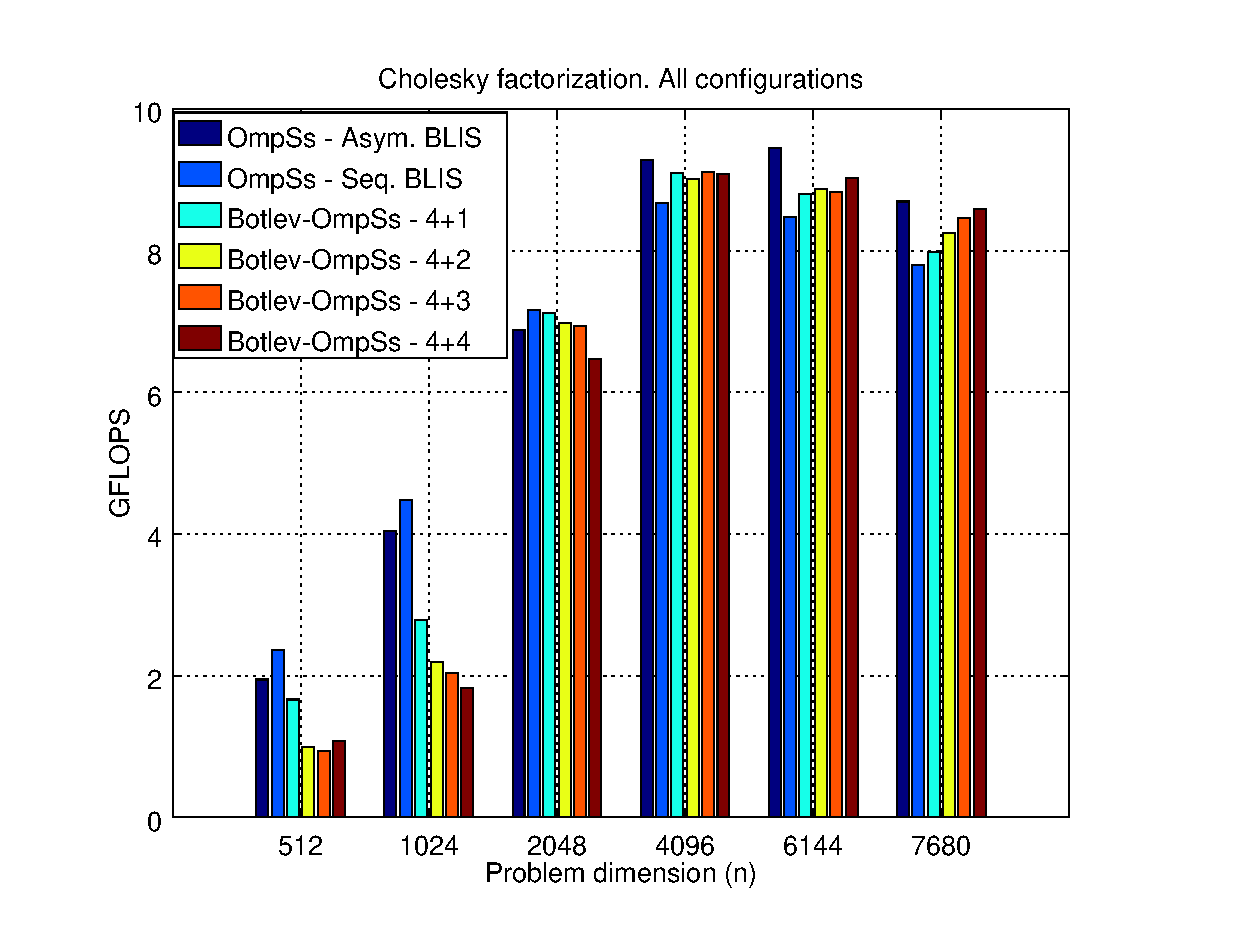
\includegraphics[width=0.70\textwidth]{Plots/Comparative/comparative}
\caption{Performance (in GFLOPS) for the Cholesky factorization using
         the conventional OmpSs runtime linked with 
         either the sequential BLIS or the multi-threaded/asymmetric BLIS, and the {\em ad-hoc} asymmetry-aware version of the
         OmpSs runtime (Botlev-OmpSs) linked with the sequential BLIS in 
         the Exynos 5422 SoC. The labels of the form ``4+x'' refer to an execution with 4 Cortex-A15 cores and x Cortex-A7 cores.}
\label{fig:comparative}
\end{figure}

To summarize, our proposal to exploit asymmetry improves portability and programmability by avoiding
a revamp of the runtime task scheduler for AMPs. In addition, our approach renders performance
gains which are, for all problems cases, comparable with those of ad-hoc asymmetry-conscious schedulers; 
for medium to large matrices, it clearly outperforms the efficiency attained with a conventional 
asymmetry-oblivious scheduler.

\subsection{Análisis detallado de rendimiento}

We next provide further details on the performance behavior of each one of the aforementioned runtime configurations.
The execution traces in this section have all been extracted with the {\tt Extrae} instrumentation
tool and analyzed with the visualization package {\tt Paraver}~\cite{Paraver}. 
The results correspond to the Cholesky factorization of a single problem with matrix dimension {\tt n}~=~6,144 and 
block size {\tt b}~=~448.

\subsubsection{General task execution overview.}

Figure~\ref{fig:traces_tasks} reports complete execution traces for each runtime configuration. 
At a glance, a number of coarse remarks can be
extracted from the trace:
\begin{itemize}
\item From the perspective of total execution time (i.e., {\em time-to-solution}), the conventional OmpSs runtime combined with 
      the asymmetric BLIS implementation attains the best results, followed by the Botlev-OmpSs runtime configuration. It is worth pointing out that
      an asymmetry-oblivious runtime which spawns 8~worker threads, with no further considerations, yields the worst performance by far. In this case, the
      load imbalance and long idle periods, especially as the amount of concurrency decreases in the final part of the trace, entail
      a huge performance penalty. 
\item The flag marks indicating task initialization/completion reveal that 
      the asymmetric BLIS implementation (which employs the combined resources from a VC) requires less time per task than 
      the two alternatives based on a sequential BLIS. An effect to note specifically in the Botlev-OmpSs configuration is the
      difference in performance between tasks of the same type, when
      executed by a big core (worker threads~5 to~8) or a LITTLE one (worker threads~1 to~4).
\item The Botlev-OmpSs task scheduler embeds a (complex) scheduling strategy that includes priorities,
      advancing the execution of tasks in the critical path and, whenever possible, assigning them to fast cores (see, for 
      example, the tasks for the factorization of diagonal blocks, 
      colored in yellow). This yields an execution timeline that is more compact during the first stages of the parallel execution, 
      at the cost of longer idle times when the degree of concurrency decreases (last iterations of the factorization). 
      Although possible, a priority-aware technique has not been applied in our experiments with the conventional OmpSs setups
      and remains part of future work.
\end{itemize}


\begin{figure}%[t]
\centering
	\begin{subfigure}{\textwidth}
   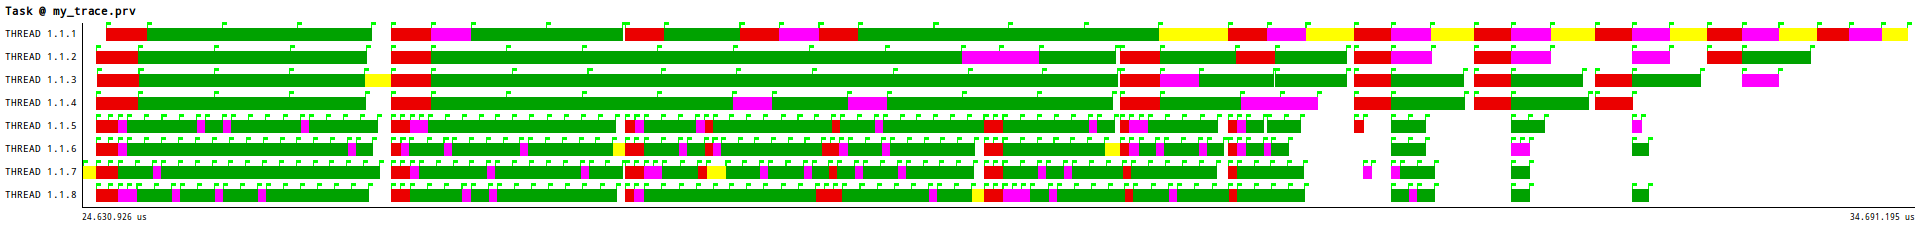
\includegraphics[width=\textwidth]{Plots/Traces/sym_8cores_tasks.png}
		\caption{OmpSs - Sequential BLIS (8 worker threads)} 
	\end{subfigure}
	\begin{subfigure}{\textwidth}
   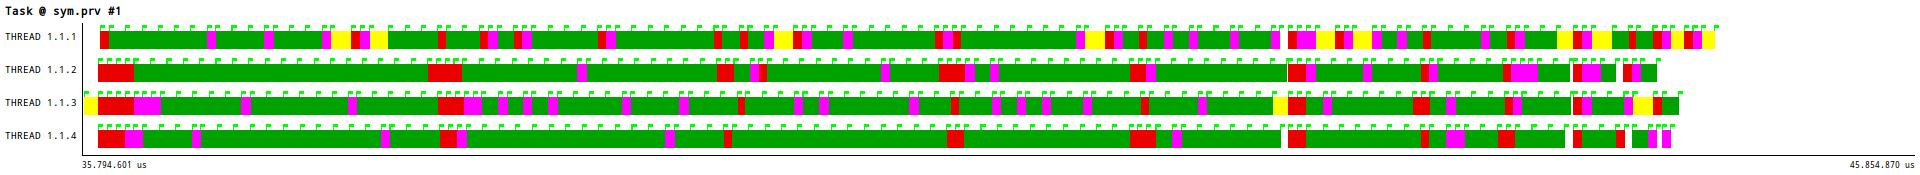
\includegraphics[width=\textwidth]{Plots/Traces/sym_tasks.png}
 \caption{OmpSs - Sequential BLIS (4 worker threads)} 
	\end{subfigure}
	\begin{subfigure}{\textwidth}
   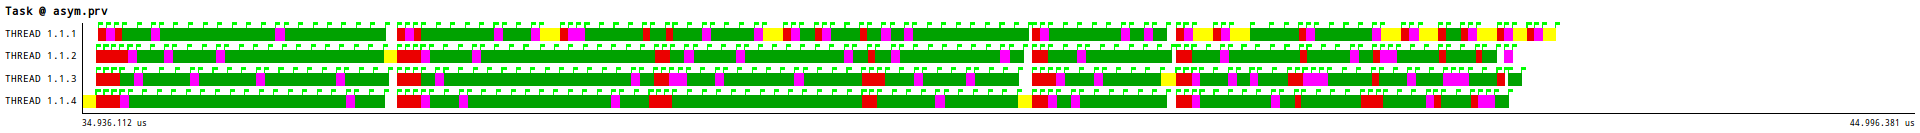
\includegraphics[width=\textwidth]{Plots/Traces/asym_tasks.png}
		\caption{OmpSs - Asymmetric BLIS (4 worker threads)}
	\end{subfigure}
	\begin{subfigure}{\textwidth}
   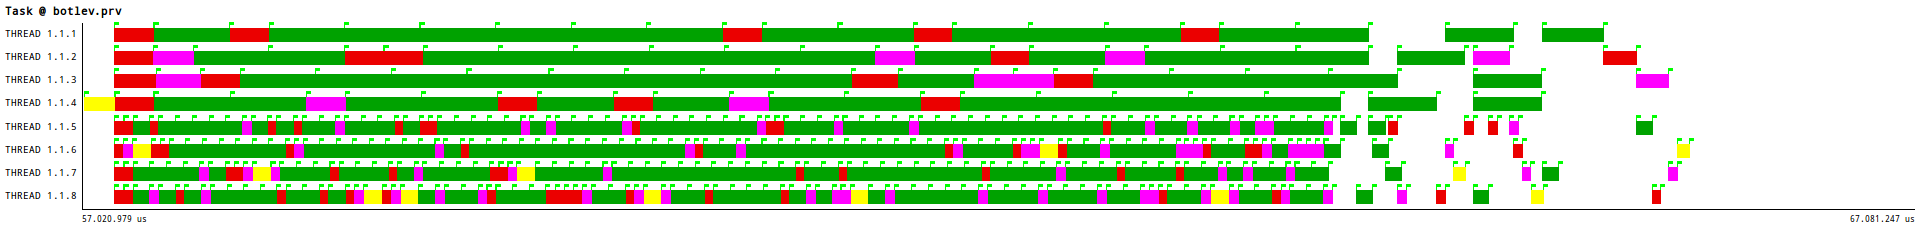
\includegraphics[width=\textwidth]{Plots/Traces/botlev_tasks.png}
		\caption{Botlev-OmpSs - Sequential BLIS (8 worker threads, 4+4)}
	\end{subfigure}
\caption{Execution traces of the three runtime configurations for the Cholesky factorization ({\tt n}~=~6,144, 
{\tt b}~=~448). 
%Task colors match with those in Figure~\ref{fig:dag}. Sections in light blue correspond to idle time. 
The timeline in each row collects the tasks executed by a single worker thread. 
Tasks are colored following the convention in Figure~\ref{fig:dag};
phases colored in white between tasks represent idle times.
The green flags mark task initialization/completion. 
%ENRIQUE, FIJATE EN VARIAS COSAS: LA DIFERENCIA EN TIEMPOS DE EJECUCION DE LAS TAREAS EN BOTLEV ENTRE LOS CUATRO PRIMEROS CORES -LENTOS- Y LOS CUATRO ULTIMOS -RAPIDOS- (he
%anyadido banderitas para que se vea mejor). MIRA
%TAMBIEN COMO ADELANTA CHOLESKY: AQUI HAY PRIORIDADES, EN LAS OTRAS DOS CONFIGURACIONES, AUNQUE PODRIA, NO LAS HAY. FIJATE TAMBIEN EN COMO BOTLEV COMPACTA
%TANTO LAS TAREAS QUE PENALIZA MUCHISIMO EN LA FASE FINAL DE LA EJECUCION, CUANDO NO QUEDA PARALELISMO. SI NO FUERA POR ESO, BARRERIA EN RENDIMIENTO AL RESTO.
}
\label{fig:traces_tasks}
\end{figure}

We next provide a quantitative analysis on the task duration and a more detailed study of 
the scheduling strategy integrated in each configuration.

\subsubsection{Task duration.}
 
Table~\ref{tab:2dp_tasks} reports the average execution time per type of task for each worker thread.
%In the conventional runtime setups, 
These results show that the execution time per individual type of task is considerably shorter
for our multithreaded/asymmetric BLIS implementation than for the alternatives based on a sequential
version of BLIS. The only exception is the factorization of the diagonal block ({\tt dpotrf}) as this is
an LAPACK-level routine, and therefore it is not available in BLIS. Inspecting the task execution time of
the Botlev-OmpSs configuration, we observe a remarkable difference depending
on the type of core tasks are mapped to. For example, the average execution times for {\tt dgemm}
range from more than 400~ms on a LITTLE core, to roughly 90~ms on a big core. This
behavior is reproduced for all types of tasks.

%To illustrate these facts, Figure~\ref{fig:traces_task_duration} represents a detailed histogram of the execution times 
%for the {\tt dgemm} task instantiations in the task-parallel executions. Each bin corresponds to the amount of tasks
%with a given execution time while rows correspond to different worker threads. Comparing conventional runtimes (traces (a) and (b)), 
%there is a clear deviation in the average execution times towards faster executions, that is, the average time to execute a task
%using the asymmetry-aware BLIS implementation is shorter. The histogram for Botlev (trace (c)) 
%exhibits two different peaks, corresponding to tasks executed on the big or on the LITTLE cores, respectively. Note that tasks executing on the fast
%cores do it at the same performance rate as those for the conventional runtime setup using a sequential BLIS implementation. 
%A similar behavior has been observed for the rest of the BLAS-3 tasks involved in the computation.

%\begin{figure}%[t]
%\centering
 %\subfigure[OmpSs + Symmetric BLIS]{
   %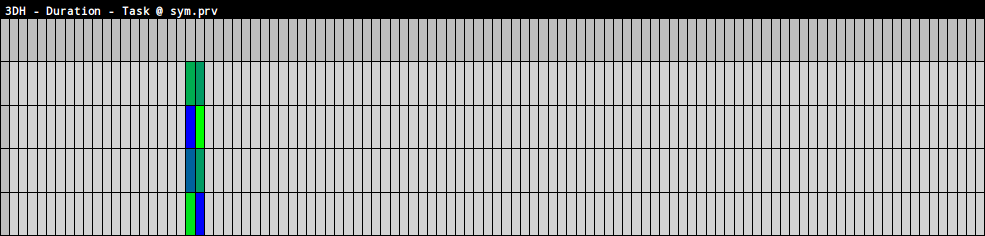
\includegraphics[width=\textwidth]{Plots/Traces/sym_task_duration_histogram.png}
%}
 %\subfigure[OmpSs + Asymmetric BLIS]{
   %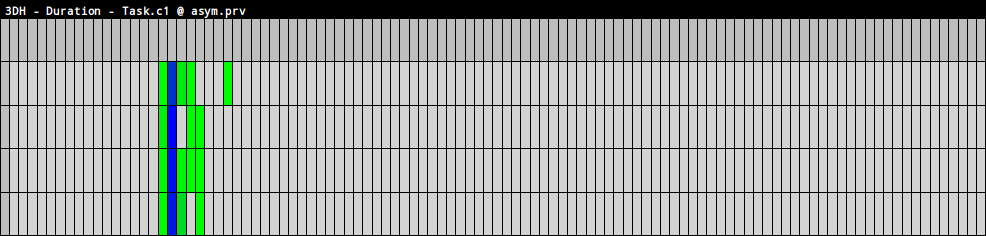
\includegraphics[width=\textwidth]{Plots/Traces/asym_task_duration_histogram.png}
%}
 %\subfigure[Botlev-OmpSs - 4+4 threads]{
   %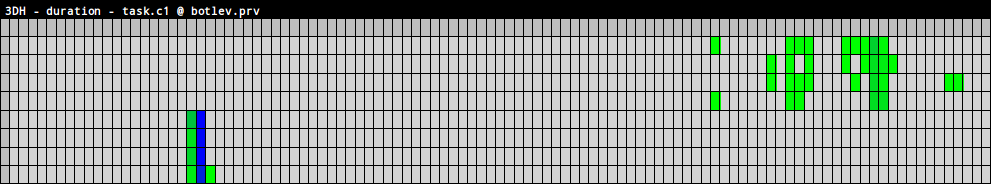
\includegraphics[width=\textwidth]{Plots/Traces/botlev_task_duration_histogram.png}
%}
%\caption{Task time duration histogram for {\tt dgemm} tasks on the three studied runtime configurations for the Cholesky factorization ({\tt n}~=~6,144, {\tt b}~=~448).  
%Rows correspond to worker threads in the execution. Columns correspond to time bins. Gradient color indicates the number of tasks in the corresponding bin (ranging
%from light green to dark blue).}
%\label{fig:traces_task_duration}
%\end{figure}


\begin{table}%[t]
\centering
\caption{Average time (in ms) per task and worker thread in the Cholesky factorization  ({\tt n}~=~6,144, 
{\tt b}~=~448), for the three runtime configurations.}
\label{tab:2dp_tasks}

\ra{1.2}
\ca{2pt}

\renewcommand{\fg}[1]{{#1}} 
\renewcommand{\br}[1]{{#1}} 

{\scriptsize
\begin{tabular}{crrrrrrrrrrrrrrr} 
   	\toprule
                 & \phantom{a} & \multicolumn{4}{c}{OmpSs - Seq. BLIS} & \phantom{ab} & \multicolumn{4}{c}{OmpSs - Asym. BLIS} & \phantom{ab} & \multicolumn{4}{c}{Botlev-OmpSs - Seq. BLIS} \\ 
                 & \phantom{a} & \multicolumn{4}{c}{(4 worker threads)} & \phantom{ab} & \multicolumn{4}{c}{(4 worker threads)} & \phantom{ab} & \multicolumn{4}{c}{(8 worker threads, 4+4)} \\ 
                                          \cmidrule{3-6}                                         \cmidrule{8-11}                                      \cmidrule{13-16}
                       & \phantom{a} &    {\tt dgemm} & {\tt dtrsm}& {\tt dsyrk}& {\tt dpotrf}  & \phantom{ab} & {\tt dgemm}  & {\tt dtrsm} & {\tt dsyrk} & {\tt dpotrf}& \phantom{ab} & {\tt dgemm} & {\tt dtrsm} & {\tt dsyrk} & {\tt dpotrf}         \\ \hline 
	 {\sc wt 0}    & \phantom{a} &    \br{89.62} & \fg{48.12} & \fg{47.14} & \fg{101.77}    & \phantom{ab} & \fg{79.82}  & \fg{42.77}  & \fg{44.42}  & \fg{105.77}  & \phantom{ab} & \fg{406.25} & \fg{216.70} & \fg{--} & \fg{--}    \\ \cline{3-16}
	 {\sc wt 1}    & \phantom{a} &    \br{88.96} & \br{48.10} & \fg{47.14} & \fg{--}      & \phantom{ab} & \fg{78.65}  & \fg{42.97}  & \fg{44.56}  & \fg{76.35}  & \phantom{ab} & \fg{408.90} & \fg{207.41} & \fg{212.55} & \fg{--}    \\ \cline{3-16}
	 {\sc wt 2}    & \phantom{a} &    \br{89.02} & \br{48.36} & \br{47.18} & \fg{87.22}    & \phantom{ab} & \fg{79.14}  & \fg{43.14}  & \fg{44.60}  & \fg{85.98}  & \phantom{ab} & \fg{415.31} & \fg{230.07} & \fg{212.56} & \fg{--}    \\ \cline{3-16}
	 {\sc wt 3}    & \phantom{a} &    \br{90.11} & \br{48.51} & \br{47.42} & \fg{--}      & \phantom{ab} & \fg{79.28}  & \fg{43.10}  & \fg{44.59}  & \fg{67.73}  & \phantom{ab} & \fg{410.84} & \fg{216.95} & \fg{216.82} & \fg{137.65}    \\ \cline{3-16}
	 {\sc wt 4}    & \phantom{a} &    \br{--} & \br{--} & \br{--} & \fg{--} & \phantom{ab} & \fg{--}  & \fg{--} & \fg{--} & \fg{--} & \phantom{ab} & \fg{90.97} & \fg{48.97} & \fg{48.36} & \fg{--}    \\ \cline{3-16}
	 {\sc wt 5}    & \phantom{a} &    \br{--} & \br{--} & \br{--} & \fg{--} & \phantom{ab} & \fg{--}  & \fg{--} & \fg{--} & \fg{--} & \phantom{ab} & \fg{90.61} & \fg{48.86} & \fg{48.16} & \fg{90.78}    \\ \cline{3-16}
	 {\sc wt 6}    & \phantom{a} &    \br{--} & \br{--} & \br{--} & \fg{--} & \phantom{ab} & \fg{--}  & \fg{--} & \fg{--} & \fg{--} & \phantom{ab} & \fg{91.28} & \fg{49.43} & \fg{47.97} & \fg{89.58}    \\ \cline{3-16}
	 {\sc wt 7}    & \phantom{a} &    \br{--} & \br{--} & \br{--} & \fg{--} & \phantom{ab} & \fg{--}  & \fg{--} & \fg{--} & \fg{--} & \phantom{ab} & \fg{91.60} & \fg{49.49} & \fg{48.62} & \fg{95.43}    \\ \bottomrule
	 %{\sc TOTAL}   & \phantom{a} &    \br{25.57} & \br{3.76} & \br{3.68} & \fg{1.24} & \phantom{ab} & \fg{22.65}  & \fg{3.35} & \fg{3.47} & \fg{1.26} & \phantom{ab} & \fg{44.07} & \fg{6.51} & \fg{6.12} & \fg{3.14}    \\ \bottomrule
	 {\sc Avg.}     & \phantom{a} &    \br{89.43} & \br{48.27} & \br{47.22} & \fg{94.49} & \phantom{ab} & \fg{79.22}   & \fg{42.99} & \fg{44.54} & \fg{83.96} & \phantom{ab} & \fg{250.72} & \fg{133.49} & \fg{119.29} & \fg{103.36}    \\ \bottomrule
\end{tabular}
}

\end{table}

\subsubsection{Task scheduling policies and idle times.}

Figure~\ref{fig:traces_task_number} illustrates the task execution order determined by the Nanos++ task scheduler. 
Here tasks are depicted using a color gradient, attending to the order in which they are encountered in the sequential code, 
from the earliest to the latest.

At runtime, the task scheduler in Botlev-OmpSs issues tasks to execution out-of-order depending on their criticality. 
The main idea behind this scheduling policy is to track the criticality of each task and, when possible, 
advance the execution of critical tasks assigning them to the fast Cortex-A15 cores. 
Conformally with this strategy, an out-of-order execution reveals itself more frequently in the timelines for the big cores 
than in those for the LITTLE cores. 
With the conventional runtime, the out-of-order execution is only dictated 
by the order in which data dependencies for tasks are satisfied.

From the execution traces, we can observe that the Botlev-OmpSs alternative suffers a remarkable
performance penalty due to the existence of idle periods in the final part of the factorization, 
when the concurrency in the factorization is greatly diminished. 
This problem is not present in the conventional scheduling policies.
In the first stages of the factorization, however, the use of a priority-aware policy for the Botlev-OmpSs scheduler
effectively reduces idle times. 
Table~\ref{tab:th_state} reports the percentage of time each worker
thread is in {\tt running} or {\tt idle} state. In general, the relative amount of time spent in idle state is much 
higher for Botlev-OmpSs than for the conventional implementations (17\% vs. 5\%, respectively). 
Note also the remarkable difference in the percentage of idle time between 
the big and LITTLE cores (20\% and ~13\%, respectively), which drives to the conclusion that the fast cores stall waiting for
completion of tasks executed on the LITTLE cores. This fact can be confirmed in the final stages of the Botlev-OmpSs trace.

The previous observations pave the road to a combination of scheduling policy and execution model for AMPs, 
in which asymmetry is exploited through {\em ad-hoc} scheduling policies during the first stages of the factorization 
--when the potential parallelism is massive--, and this is later replaced with the use 
of asymmetric-aware kernels and coarse-grain VCs
in the final stages of the execution, when the concurrency is scarce. Both approaches are not mutually exclusive, 
but complementary depending on the level of task concurrency available at a given execution stage.

\begin{figure}%[t]
\centering
	\begin{subfigure}{\textwidth}
   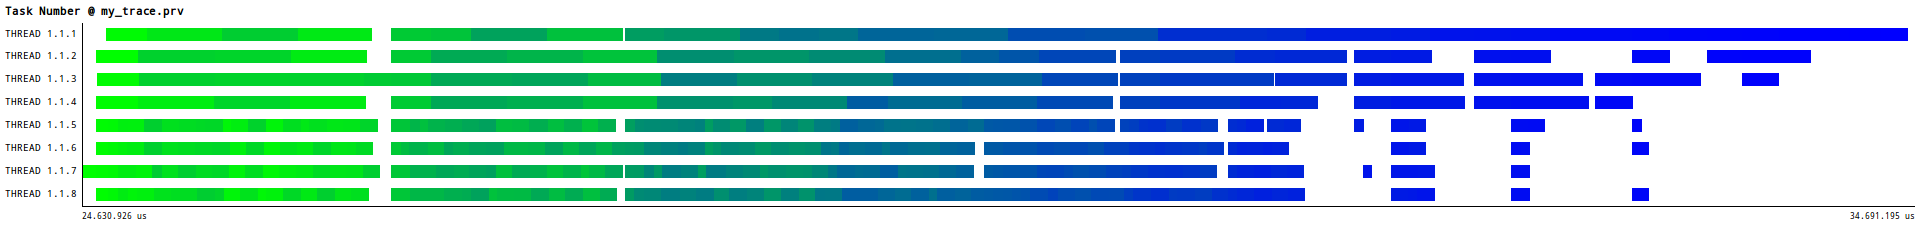
\includegraphics[width=\textwidth]{Plots/Traces/sym_8cores_task_number.png}
		\caption{OmpSs - Sequential BLIS (8 worker threads)}
	\end{subfigure}
	\begin{subfigure}{\textwidth}
   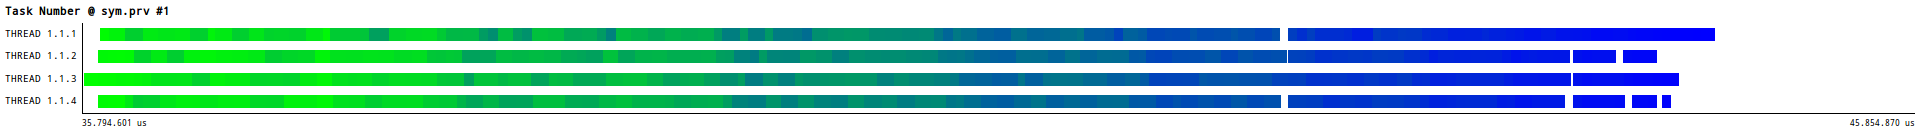
\includegraphics[width=\textwidth]{Plots/Traces/sym_task_number.png}
		\caption{OmpSs - Sequential BLIS (4 worker threads)} 
	\end{subfigure}
	\begin{subfigure}{\textwidth}
   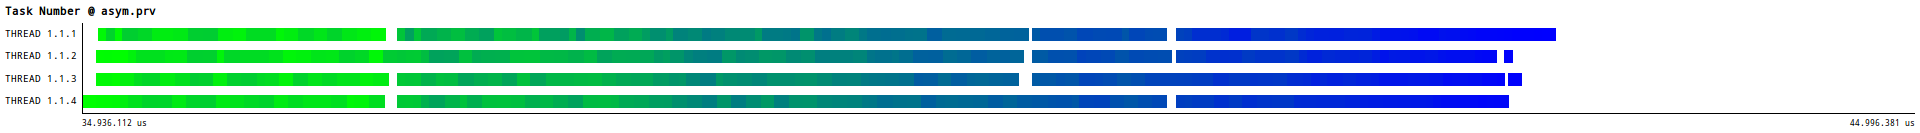
\includegraphics[width=\textwidth]{Plots/Traces/asym_task_number.png}
		\caption{OmpSs - Asymmetric BLIS (4 worker threads)} 
	\end{subfigure}
	\begin{subfigure}{\textwidth}
   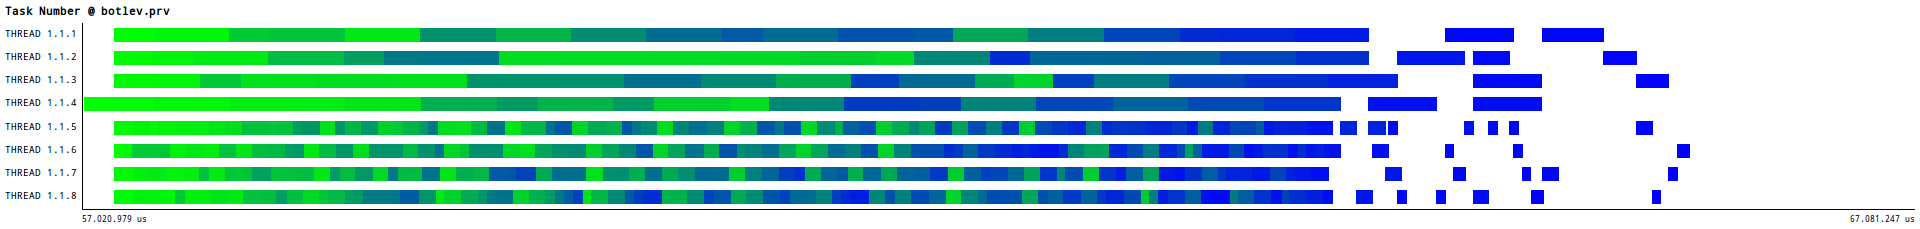
\includegraphics[width=\textwidth]{Plots/Traces/botlev_task_number.png}
		\caption{Botlev-OmpSs - Sequential BLIS (8 worker threads, 4+4)} 
	\end{subfigure}
\caption{Task execution order of the three studied runtime configurations for the Cholesky factorization 
({\tt n}~=~6,144, {\tt b}~=~448). In the trace, tasks are ordered
according to their appearance in the sequential code, 
and depicted using a color gradient, with light green indicating early tasks, and dark blue for the late
tasks. 
%ENRIQUE, FIJATE COMO SE NOTA
%MAS LA EJECUCION FUERA DE ORDEN EN BOTLEV, ESPECIALMENTE EN LOS CORES RAPIDOS (Y MIRA POR EJEMPLO COMO ADELANTA CHOLESKY). BOTLEV USA PRIORIDADES. LAS OTRAS DOS CONFIGURACIONES, AUNQUE PODRIAN, NO LO HACEN EN NUESTRA CONFIGURACION, LO CUAL
%ES UN PUNTO A FAVOR.
}
\label{fig:traces_task_number}
\end{figure}

\begin{table}
\centering
\caption{Percentage of time per worker thread in idle or running state for different runtime configurations for the Cholesky factorization 
({\tt n}~=~6,144, {\tt b}~=~448).
Note that {\sc wt 0} is the master thread, and thus is never idle; for it, the rest of the time till
100\% percentage is devoted to {\tt synchronization}, {\tt scheduling} and {\tt thread creation}. For the rest of threads, this amount of time is devoted to {\tt runtime overhead}.}
\label{tab:th_state}

\ra{1.2}
\ca{2pt}

\renewcommand{\fg}[1]{{#1}} 
\renewcommand{\br}[1]{{#1}} 

{\scriptsize
\begin{tabular}{crrrrrrrrr} 
   	\toprule
                 & \phantom{a} & \multicolumn{2}{c}{OmpSs - Seq. BLIS} & \phantom{ab} & \multicolumn{2}{c}{OmpSs - Asym. BLIS} & \phantom{ab} & \multicolumn{2}{c}{Botlev-OmpSs - Seq. BLIS} \\ 
                 & \phantom{a} & \multicolumn{2}{c}{(4 worker threads)} & \phantom{ab} & \multicolumn{2}{c}{(4 worker threads)} & \phantom{ab} & \multicolumn{2}{c}{(8 worker threads, 4+4)} \\ 
                 %& \phantom{a} & \multicolumn{4}{c}{OmpSs - Seq. BLIS} & \phantom{ab} & \multicolumn{4}{c}{OmpSs - Asym. BLIS} & \phantom{ab} & \multicolumn{4}{c}{Botlev-OmpSs - Seq. BLIS} \\ 
                 %& \phantom{a} & \multicolumn{4}{c}{(4 worker threads)} & \phantom{ab} & \multicolumn{4}{c}{(4 worker threads)} & \phantom{ab} & \multicolumn{4}{c}{(8 worker threads, 4+4)} \\ 
                                          \cmidrule{3-4}                                         \cmidrule{6-7}                                      \cmidrule{9-10}
                       & \phantom{a} &    {\tt idle}& {\tt running}& \phantom{ab}  & {\tt idle}& {\tt running}& \phantom{ab} & {\tt idle}  & {\tt running} \\ \hline 
	 {\sc wt 0}    & \phantom{a} &    \fg{--}   & \fg{98.41}   & \phantom{ab}  & \fg{--}   & \fg{97.85}   & \phantom{ab} & \fg{--}     & \fg{86.53}    \\ \cline{3-10}
	 {\sc wt 1}    & \phantom{a} &    \br{5.59} & \fg{94.22}   & \phantom{ab}  & \fg{5.51} & \fg{94.29}   & \phantom{ab} & \fg{13.63}  & \fg{86.28}    \\ \cline{3-10}
	 {\sc wt 2}    & \phantom{a} &    \br{3.14} & \fg{96.67}   & \phantom{ab}  & \fg{5.27} & \fg{94.53}   & \phantom{ab} & \fg{13.94}  & \fg{85.98}    \\ \cline{3-10}
	 {\sc wt 3}    & \phantom{a} &    \br{5.77} & \fg{94.07}   & \phantom{ab}  & \fg{5.17} & \fg{94.62}   & \phantom{ab} & \fg{13.43}  & \fg{86.47}    \\ \cline{3-10}
	 {\sc wt 4}    & \phantom{a} &    \br{--}   & \fg{--}      & \phantom{ab}  & \fg{--}   & \fg{--}      & \phantom{ab} & \fg{19.26}  & \fg{80.51}    \\ \cline{3-10}
	 {\sc wt 5}    & \phantom{a} &    \br{--}   & \fg{--}      & \phantom{ab}  & \fg{--}   & \fg{--}      & \phantom{ab} & \fg{21.12}  & \fg{78.69}    \\ \cline{3-10}
	 {\sc wt 6}    & \phantom{a} &    \br{--}   & \fg{--}      & \phantom{ab}  & \fg{--}   & \fg{--}      & \phantom{ab} & \fg{20.84}  & \fg{78.97}    \\ \cline{3-10}
	 {\sc wt 7}    & \phantom{a} &    \br{--}   & \fg{--}      & \phantom{ab}  & \fg{--}   & \fg{--}      & \phantom{ab} & \fg{20.09}  & \fg{79.70}    \\ \bottomrule
	 %{\sc TOTAL}   & \phantom{a} &    \br{13.87} & \fg{384.31}    & \phantom{ab}  & \fg{16.97}  & \fg{379.60}    & \phantom{ab} & \fg{73.81}  & \fg{715.16}   \\ \bottomrule
	 {\sc Avg.}     & \phantom{a} &    \br{4.84} & \fg{95.89}    & \phantom{ab} & \fg{5.32} & \fg{94.90}   & \phantom{ab} & \fg{17.47}  & \fg{82.89}    \\ \bottomrule
\end{tabular}
}

\end{table}



%-- Configuraciones para emacs --
%%% Local Variables:
%%% mode: latex
%%% TeX-master: "./principal.tex"
%%% End:
